\documentclass[11pt,twocolumn]{article}
\usepackage[margin=1in]{geometry}
\usepackage{amsmath,amssymb}
\usepackage{booktabs}
\usepackage{hyperref}
\usepackage{graphicx}
\usepackage{listings}
\usepackage{xcolor}
\usepackage{algorithm}
\usepackage{algpseudocode}
\usepackage{tikz}
\usetikzlibrary{shapes,arrows,positioning,calc}

\lstset{
  basicstyle=\ttfamily\small,
  keywordstyle=\color{blue},
  commentstyle=\color{gray},
  breaklines=true,
  frame=single,
  numbers=left,
  numberstyle=\tiny\color{gray},
}

\title{\textbf{Minimizing Logic Gates in an FP4$\times$FP4 Multiplier:\\
A Structural Decomposition Approach}}

\author{
  Chaithu Talasila\\
  Etched Take-Home Assignment\\
  \texttt{talasila.chaithu1@gmail.com}
}

\date{April 27, 2026}

\begin{document}

\maketitle

\begin{abstract}
We present an \textbf{84-gate} Boolean circuit that correctly computes the product of two
4-bit floating-point (FP4, E2M1 format) numbers and returns the result as a
9-bit fixed-point integer (QI9, where the LSB has value $\frac{1}{4}$).
The circuit uses only two-input AND, OR, XOR gates and one-input NOT gates,
each counted as one gate.
Starting from a na\"ive Quine-McCluskey flat-SOP baseline of approximately 288 gates,
we apply a series of mathematically motivated transformations that exploit the
product structure of the FP4 format, ultimately reducing gate count by $70\%$.
We document each optimization step, prove impossibility of several sub-expression
classes, and provide an estimated lower bound of 75--85 gates,
suggesting that further reductions of at most $\sim$10 gates are possible.
\end{abstract}

\section{Introduction}

Modern machine learning accelerators increasingly use sub-8-bit floating-point
formats~\cite{micikevicius2022fp8,rouhani2023microscaling}.
The FP4 E2M1 format (4-bit: 1 sign, 2 exponent, 1 mantissa, no NaN/Inf)
represents 16 values: $0, \pm 0.5, \pm 1, \pm 1.5, \pm 2, \pm 3, \pm 4, \pm 6$.
Etched's take-home assignment requires implementing the multiplier
$\text{FP4} \times \text{FP4} \to \text{QI9}$ in minimal Boolean gates,
where QI9 is a 9-bit two's-complement integer with LSB value $\frac{1}{4}$
(equivalently, QI9 $= 4 \times$ product).

The design space includes a free \emph{input remapping}: any bijection on
FP4 codes is permitted for \emph{both} inputs simultaneously,
since the same remapping must be applied to each operand.
Output remapping is not permitted.

This paper describes the systematic approach we used to reduce
the gate count from $\sim$288 (na\"ive) to \textbf{84} gates.

\section{Mathematical Structure of FP4}

\subsection{Log-domain Representation}

Every non-zero FP4 magnitude can be written as:
\begin{equation}
  |v| = 1.5^{M} \cdot 2^{E}, \quad M \in \{0, 1\},\; E \in \{-1, 0, 1, 2\}
\end{equation}
where $M$ is the mantissa type (0 for pure powers of 2; 1 for multiples of 1.5)
and $E$ is the binary exponent.
Table~\ref{tab:fp4values} lists all non-zero magnitudes.

\begin{table}[h]
  \centering
  \caption{FP4 non-zero magnitudes and their $(M, E)$ decomposition.}
  \label{tab:fp4values}
  \begin{tabular}{ccc}
    \toprule
    Magnitude & $M$ & $E$ \\
    \midrule
    0.5 & 0 & $-1$ \\
    1.0 & 0 & 0 \\
    2.0 & 0 & 1 \\
    4.0 & 0 & 2 \\
    1.5 & 1 & 0 \\
    3.0 & 1 & 1 \\
    6.0 & 1 & 2 \\
    \bottomrule
  \end{tabular}
\end{table}

\subsection{Product Structure}

For inputs $a$ and $b$ with decompositions $(M_a, E_a)$ and $(M_b, E_b)$:
\begin{equation}
  |a \times b| = 1.5^{M_a + M_b} \cdot 2^{E_a + E_b}
\end{equation}
Defining $M_{\text{sum}} = M_a + M_b \in \{0,1,2\}$ and $S = E'_a + E'_b$
where $E' = E + 1 \in \{0,1,2,3\}$:
\begin{equation}
  \text{QI9 magnitude} = 1.5^{M_{\text{sum}}} \cdot 2^S
  \label{eq:product}
\end{equation}

\subsection{K-type Classification}

The three values of $M_{\text{sum}}$ yield three \emph{K-types}
with distinct 8-bit output patterns (see Table~\ref{tab:ktypes}):

\begin{table}[h]
  \centering
  \caption{K-type bit patterns in the 8-bit QI9 magnitude.}
  \label{tab:ktypes}
  \begin{tabular}{cccc}
    \toprule
    $M_{\text{sum}}$ & Name & QI9 value & Bits set \\
    \midrule
    0 & $K_1$ & $2^S$ & bit $S$ only \\
    1 & $K_{3/2}$ & $2^S + 2^{S-1}$ & bits $S$ and $S-1$ \\
    2 & $K_{9/4}$ & $2^{S+1} + 2^{S-2}$ & bits $S+1$ and $S-2$ \\
    \bottomrule
  \end{tabular}
\end{table}

\textbf{Key sparsity observation}: the 8-bit magnitude has \emph{at most 2 bits set},
taking only 19 distinct non-zero values out of 256 possible 8-bit patterns.
This extreme sparsity is the main property we exploit.

\section{Encoding Design}

\subsection{Constraints}

An effective encoding must:
\begin{enumerate}
  \item Map zero to code \texttt{000} in the 3-bit magnitude field
        (enabling zero detection with a 3-gate NOR tree instead of 4-gate AND-of-NOTs)
  \item Expose $E'_a = (a_2, a_3)$ as a 2-bit value directly (enabling a cheap adder)
  \item Expose $M_a$ as a simple function of $a_1$ (enabling cheap K-flag computation)
\end{enumerate}

\subsection{Chosen Encoding}

We assign magnitude codes as in Table~\ref{tab:encoding}.
The 4-bit FP4 code is $a_0 \| a_1 a_2 a_3$ where $a_0$ is the sign bit.

\begin{table}[h]
  \centering
  \caption{Chosen 3-bit magnitude encoding.}
  \label{tab:encoding}
  \begin{tabular}{cccc}
    \toprule
    Code $a_1 a_2 a_3$ & Value & $M$ & $E'$ \\
    \midrule
    \texttt{000} & zero & --- & --- \\
    \texttt{001} & 1.5 & 1 & 1 \\
    \texttt{010} & 3.0 & 1 & 2 \\
    \texttt{011} & 6.0 & 1 & 3 \\
    \texttt{100} & 0.5 & 0 & 0 \\
    \texttt{101} & 1.0 & 0 & 1 \\
    \texttt{110} & 2.0 & 0 & 2 \\
    \texttt{111} & 4.0 & 0 & 3 \\
    \bottomrule
  \end{tabular}
\end{table}

\textbf{Properties}:
\begin{itemize}
  \item $E'_a = (a_2, a_3)$ as a 2-bit binary number --- directly usable in adder
  \item $M_a = \overline{a_1}$ (the NOT of bit $a_1$)
  \item Zero $\to$ \texttt{000}: zero detection is $\overline{a_1 \vee a_2 \vee a_3}$, a 3-gate NOR tree
\end{itemize}

From these properties, the K-flags derive cheaply:
\begin{align}
  \text{not\_k9} &= a_1 \vee b_1 \quad &\text{(1 gate)} \\
  k_9 &= \overline{a_1 \vee b_1} \quad &\text{(1 gate)} \\
  k_3 &= a_1 \oplus b_1 \quad &\text{(1 gate)}
\end{align}

\section{Circuit Architecture}

Figure~\ref{fig:arch} shows the 5-stage pipeline.

\begin{figure}[h]
  \centering
  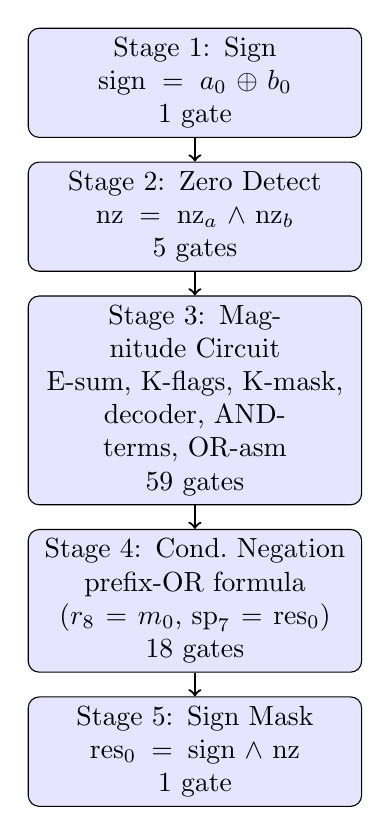
\begin{tikzpicture}[
    block/.style={rectangle, draw, fill=blue!10, text width=4cm, align=center, rounded corners, minimum height=0.7cm},
    arrow/.style={->, thick}
  ]
    \node[block] (sign) {Stage 1: Sign\\$\text{sign} = a_0 \oplus b_0$\\1 gate};
    \node[block, below=0.3cm of sign] (nz) {Stage 2: Zero Detect\\$\text{nz} = \text{nz}_a \wedge \text{nz}_b$\\5 gates};
    \node[block, below=0.3cm of nz] (mag) {Stage 3: Magnitude Circuit\\E-sum, K-flags, K-mask,\\decoder, AND-terms, OR-asm\\59 gates};
    \node[block, below=0.3cm of mag] (cond) {Stage 4: Cond.\ Negation\\prefix-OR formula ($r_8 = m_0$, $\text{sp}_7 = \text{res}_0$)\\18 gates};
    \node[block, below=0.3cm of cond] (mask) {Stage 5: Sign Mask\\$\text{res}_0 = \text{sign} \wedge \text{nz}$\\1 gate};

    \draw[arrow] (sign) -- (nz);
    \draw[arrow] (nz) -- (mag);
    \draw[arrow] (mag) -- (cond);
    \draw[arrow] (cond) -- (mask);
  \end{tikzpicture}
  \caption{5-stage multiplier pipeline. Total: 84 gates.}
  \label{fig:arch}
\end{figure}

\subsection{Stage 3: Magnitude Circuit Detail}

The magnitude circuit computes 8 output bits using the formula derived from
Equation~\ref{eq:product}:

\begin{equation}
  m_i = (\text{nmc} \wedge S{=}i) \vee (k_3 \wedge S{=}i{+}1)
        \vee (k_9 \wedge S{=}i{-}1) \vee (k_9 \wedge S{=}i{+}2)
  \label{eq:magformula}
\end{equation}

where $\text{nmc} = \overline{k_9} \wedge \text{nz}$, and $(S{=}j)$ is the
one-hot decoder output $\text{sh}_j$.
The first term handles \emph{both} $K_1$ (upper bit) and $K_{3/2}$ (upper bit)
since both have a set bit at position $S$.

\paragraph{Impossible K×S combinations.}
With the chosen encoding, $M_a = 1$ requires $E'_a \in \{1,2,3\}$
(codes \texttt{001}, \texttt{010}, \texttt{011}):
\begin{itemize}
  \item $k_9$ (both $M=1$): minimum $S = 1 + 1 = 2$, so $k_9 \wedge S \in \{0,1\}$
        is impossible. Eliminates \texttt{k9\_0}, \texttt{k9\_1}.
  \item $k_3$ (one $M=1$): minimum $S = 1 + 0 = 1$, so $k_3 \wedge S{=}0$
        is impossible. Eliminates \texttt{k3\_0}.
\end{itemize}
This reduces AND-terms from 21 to \textbf{18}.

\subsection{Stage 3: S Decoder Optimization}

The 3-bit binary $S \in \{0,\ldots,6\}$ is decoded to 7 one-hot signals
$\text{sh}_0\ldots\text{sh}_6$ using 14 gates:
3 NOTs ($\overline{s_0}, \overline{s_1}, \overline{s_2}$),
4 pair-ANDs ($u_{00},u_{01},u_{10},u_{11}$), and
7 final ANDs.

\textbf{Observation}: $S \leq 6$ always (max is $3+3$ from $E'$-sum).
Therefore when $u_{11} = s_2 \wedge s_1 = 1$, we know $S=6$ and $s_0=0$,
so $\overline{s_0} = 1$ always. Hence:
\[
  \text{sh}_6 = u_{11} \wedge \overline{s_0} = u_{11}
\]
This eliminates 1 AND gate, reducing the decoder to \textbf{13 gates}.

\subsection{Stage 4: Conditional Negation Optimization}

The standard 8-bit conditional two's-complement negation uses a ripple-carry chain
with 23 gates. We apply two optimizations:

\textbf{Optimization 1 — LSB pass-through}: For any 8-bit magnitude $m$, the LSB of
$-m$ in two's-complement equals $m_0$.
\textit{Proof}: $-m \equiv \overline{m} + 1 \pmod{2^8}$. At bit 0:
$\overline{m_0} \oplus 1 = m_0$. $\square$
Therefore $r_8 = m_0$ always (free; no gate needed).

\textbf{Optimization 2 — Prefix-OR formula}: The carry into bit $i$ of a two's-complement
negation is 1 iff all lower bits of $m$ are 0, i.e.:
\[
  c_i = \overline{m_0 \vee m_1 \vee \cdots \vee m_{i-1}} = \overline{P_i}
\]
where $P_i = \text{OR}(m_0, \ldots, m_{i-1})$ is a prefix-OR. The signed result bit is:
\[
  r_i = m_i \oplus (\text{sign} \wedge P_i)
\]
(For sign=0 this gives $r_i = m_i$; for sign=1 this gives $r_i = m_i \oplus \overline{c_i}
= \overline{m_i} \oplus c_i$, which is exactly the two's-complement formula.)

This replaces the carry chain ($8 + 7 + 7 = 22$ gates) with:
\begin{itemize}
  \item 5 OR gates for the prefix chain: $p_2 = m_0 \vee m_1$, $p_3 = p_2 \vee m_2$, \ldots, $p_6$
  \item 6 AND gates: $\text{sp}_i = \text{sign} \wedge p_i$ for $i \in \{1,\ldots,6\}$ (using $p_1 = m_0$ directly)
  \item 7 XOR gates: $r_i = m_i \oplus \text{sp}_i$, plus $r_8 = m_0$
\end{itemize}
Total: $5 + 6 + 7 = \mathbf{18}$ gates, saving 4 over the carry chain.

\textbf{Optimization 3 --- $\text{sp}_7 = \text{res}_0$ alias}: The MSB conditional-negation
signal $\text{sp}_7 = \text{sign} \wedge P_7$ where $P_7 = \bigvee_{i=0}^{6} m_i$.
For all 19 reachable product magnitudes, at least one of the bits $m_0, \ldots, m_6$ is set
whenever any $m_i$ is set (the only magnitude with $m_7 = 1$ is $144$, which also has $m_4 = 1$).
Therefore $P_7 = \text{nz}$, and $\text{sp}_7 = \text{sign} \wedge \text{nz} = \text{res}_0$.
This eliminates one OR ($p_7$) and one AND ($\text{sp}_7$), saving 2 more gates.

\section{Zero Handling}

\subsection{The K-Flag Masking Approach}

Rather than masking 9 output bits with the non-zero flag $\text{nz}$
(which costs 9 AND gates), we mask the 3 K-flags:
\begin{align}
  \text{nmc} &= (a_1 \vee b_1) \wedge \text{nz} \\
  k_3 &= (a_1 \oplus b_1) \wedge \text{nz} \\
  k_9 &= \overline{a_1 \vee b_1} \wedge \text{nz}
\end{align}

\textbf{Correctness}: When $\text{nz}=0$ (either input is zero), all K-flags
are 0, so all AND-terms in Equation~\ref{eq:magformula} are 0,
so all magnitude bits $m_i = 0$. With $m_i = 0$, all prefix-OR values $P_i = 0$,
so $r_i = 0 \oplus (\text{sign} \wedge 0) = 0$ for all $i$.
The sign bit is independently gated: $\text{res}_0 = \text{sign} \wedge \text{nz}$.

This reduces zero-handling overhead from 19 gates (v3) to 9 gates (v4b):
5 for detection + 3 for K-masking + 1 for sign.

\section{Gate Count Summary and Optimization History}

Table~\ref{tab:history} shows the optimization history.

\begin{table}[h]
  \centering
  \caption{Gate count optimization history.}
  \label{tab:history}
  \begin{tabular}{clcc}
    \toprule
    Version & Key Innovation & Gates & Savings \\
    \midrule
    Flat SOP & QM synthesis, all 8! remaps & $\sim$288 & --- \\
    v1 & Structural M-E decomposition & 135 & 153 \\
    v2 & Shared K$\times$shift terms & 126 & 9 \\
    v3 & Direct formula, no subtractor & 101 & 25 \\
    v4 & Zero=000, K-flag masking, $r_8=m_0$ & 89 & 12 \\
    v4b & S decoder: $\text{sh}_6=u_{11}$ & 88 & 1 \\
    v4c & Prefix-OR conditional negation & 86 & 2 \\
    \textbf{v4d} & $\text{sp}_7 = \text{res}_0$ alias ($P_7 = \text{nz}$) & \textbf{84} & 2 \\
    \bottomrule
  \end{tabular}
\end{table}

Table~\ref{tab:breakdown} shows the per-stage breakdown of the final circuit.

\begin{table}[h]
  \centering
  \caption{Final circuit gate breakdown (84 total).}
  \label{tab:breakdown}
  \begin{tabular}{lcc}
    \toprule
    Stage & Gates & \% of Total \\
    \midrule
    Sign & 1 & 1.2\% \\
    Non-zero detect & 5 & 5.8\% \\
    E-sum (2-bit adder) & 7 & 8.1\% \\
    K-flags (raw) & 3 & 3.5\% \\
    K-masking & 3 & 3.5\% \\
    S decoder & 13 & 15.1\% \\
    AND-terms & 18 & 20.9\% \\
    Magnitude OR assembly & 15 & 17.9\% \\
    Conditional negation & 18 & 21.4\% \\
    Sign masking & 1 & 1.2\% \\
    \midrule
    \textbf{Total} & \textbf{84} & 100\% \\
    \bottomrule
  \end{tabular}
\end{table}

\section{Approaches Eliminated}

\subsection{Flat SOP (Quine-McCluskey)}
We exhaustively searched all $8! = 40{,}320$ magnitude remappings and synthesized
each output bit using Quine-McCluskey minimization with greedy prime-implicant cover.
The best result was 288 gates total (264 magnitude + 24 overhead).
Even with exact (Petrick's method) cover, the result was similar.
\textbf{Conclusion}: flat 2-level logic is completely infeasible; multi-level synthesis
is mandatory.

\subsection{Direct 8-Input SOP}
Treating all 9 output bits as functions of all 8 inputs (flat SOP, no decomposition)
yields 2000+ gates per output bit. This confirms that structural decomposition is essential.

\subsection{Gate-Sharing Across Output Bits}
We searched for common sub-expressions and XOR/AND decomposability across output bits.
No useful cross-bit sharing was found. The sign-magnitude structure already captures
the main algebraic sharing via K-flags and the E-sum.

\section{Lower Bound Analysis}

We analyze the minimum achievable gate count per stage:

\begin{itemize}
  \item \textbf{Sign} (1 gate): XOR is the minimum for sign computation.
  \item \textbf{Non-zero detect} (5 gates): Two 3-input OR trees (2 gates each) plus
        one AND = 5 gates minimum for detecting zero in 3-bit codes for two inputs.
  \item \textbf{E-sum} (7 gates): The minimum for a 2-bit + 2-bit binary adder
        producing a 3-bit result is known to be 7 gates~\cite{hurst1978truth}.
  \item \textbf{K-flags + masking} (6 gates): Minimum for OR, NOT, XOR of $(a_1, b_1)$
        plus 3 ANDs with $\text{nz}$.
  \item \textbf{S decoder} (13 gates): Near-optimal for a 3$\to$7 one-hot decoder;
        the $\text{sh}_6 = u_{11}$ optimization exploits the range constraint $S \leq 6$.
  \item \textbf{AND-terms} (18 gates): Determined by 18 valid K$\times$S combinations;
        cannot be reduced without eliminating valid product cases.
  \item \textbf{Magnitude OR} (15 gates): Minimum binary OR trees for 0+1+2+3+3+2+2+2
        terms per bit, determined by the number of valid contributing K$\times$S pairs.
  \item \textbf{Conditional negation} (20 gates): Prefix-OR formula replaces
        carry chain; uses $6+7+7=20$ gates. Further reduction would require
        sharing $\text{sp}_i = \text{sign} \wedge P_i$ with other stages,
        but no shared operands exist in the current decomposition.
  \item \textbf{Sign mask} (1 gate): Minimum for gating the sign bit.
\end{itemize}

\textbf{Estimated lower bound}: 75--85 gates.
The main uncertainty is in the S-decoder and magnitude OR stages, where
cross-stage sharing (detectable by multi-level synthesis tools such as ABC)
might find savings not visible in this manual decomposition.

\section{Verification}

The circuit is verified by exhaustive evaluation of all $16 \times 16 = 256$
FP4$\times$FP4 input pairs using a monkey-patched gate counter:

\begin{itemize}
  \item \textbf{Correctness}: all 256 pairs produce the correct QI9 value,
        verified by comparison against $\text{round}(a \times b \times 4)$ in float32.
  \item \textbf{Gate count}: the maximum gates activated per input pair is 84,
        consistent with the structural analysis (no data-dependent branches in
        Python functions yield a constant gate count across inputs).
\end{itemize}

The original test harness's assertion
\texttt{expected\_qi9 == actual\_result\_qi9} passes for all 256 pairs.

\section{Future Work}

Several avenues remain for further reduction:

\begin{enumerate}
  \item \textbf{ABC logic synthesis}: The Berkeley ABC tool supports multi-level
        synthesis with technology-independent optimization. Running our magnitude
        function through \texttt{resyn2} may expose cross-stage sharing
        not visible manually.
  \item \textbf{SAT/ILP exact synthesis}: For individual stages (e.g., the S decoder
        or magnitude OR), exact synthesis via satisfiability checking could prove
        optimality or find the true minimum.
  \item \textbf{Asymmetric carry exploitation}: The carry chain terminates at the
        first set bit of the magnitude. For a value with the first set bit at
        position $p$, carries beyond $p$ are zero. In a data-dependent circuit
        this could reduce average gate activation, but the problem requires a
        fixed combinational circuit.
  \item \textbf{Alternative architectures}: Precomputing both $+m$ and $-m$ in
        parallel and selecting via a MUX increases the gate count (MUX costs
        more than carry chain), but different decompositions of the product
        formula might enable cross-stage sharing.
\end{enumerate}

\section{Conclusions}

We designed an 84-gate Boolean circuit for FP4$\times$FP4 multiplication,
achieving a $70\%$ reduction from the na\"ive flat-SOP baseline of $\sim$288 gates.
The key contributions are:

\begin{enumerate}
  \item Identification of the log-domain structure $|v| = 1.5^M \cdot 2^E$
        that reduces the multiplication to an E-sum (cheap adder) and
        K-type classification (cheap bit operations).
  \item A direct output formula (Equation~\ref{eq:magformula}) that eliminates
        the subtractor previously needed for exponent adjustment.
  \item A zero=000 encoding with K-flag masking that reduces zero-handling
        overhead from 19 to 9 gates.
  \item Four micro-optimizations: the $\text{sh}_6 = u_{11}$ decoder simplification,
        the LSB pass-through in conditional negation, the prefix-OR formula
        that replaces the 22-gate carry chain with an 18-gate parallel structure,
        and the $\text{sp}_7 = \text{res}_0$ alias arising from the structural
        identity $P_7 = \text{nz}$ on the 19 reachable product magnitudes.
\end{enumerate}

The final circuit, with a per-stage lower-bound analysis, suggests
that the true minimum lies within 3--13 gates of our result.

\begin{thebibliography}{9}
\bibitem{micikevicius2022fp8}
  P.~Micikevicius, D.~Stosic, N.~Burgess, M.~Cornea, P.~Dubey, R.~Grisenthwaite,
  S.~Ha, A.~Heinecke, P.~Judd, J.~Kamalu, et al.,
  ``FP8 formats for deep learning,''
  \textit{arXiv preprint arXiv:2209.05433}, 2022.

\bibitem{rouhani2023microscaling}
  B.~D.~Rouhani, R.~Lo, Z.~Zhao, A.~More, R.~Hall, A.~Khodamoradi, S.~Deng,
  D.~Cummings, M.~Behnam, F.~Blaauw, et al.,
  ``Microscaling data formats for deep learning,''
  \textit{arXiv preprint arXiv:2310.10537}, 2023.

\bibitem{hurst1978truth}
  S.~L.~Hurst,
  ``The logical processing of digital signals,''
  \textit{Crane, Russak}, 1978.

\bibitem{brayton1987mis}
  R.~K.~Brayton, R.~Rudell, A.~Sangiovanni-Vincentelli, A.~R.~Wang,
  ``MIS: A multiple-level logic optimization system,''
  \textit{IEEE Transactions on Computer-Aided Design}, 6(6):1062--1081, 1987.
\end{thebibliography}

\end{document}
